\chapter{Limits, colimits, and adjunctions}
Hi! This is 18.906. I'm glad to see familiar faces, and new faces. Let me introduce the course. It's a pset based course, with 6 psets. The first one is due Feb 22. It's due every two weeks, so I can't formulate all porblems right at the beginning of the two weeks. I'll try to have the psets done a week before the psets are due. So the first couple problems are up for this pset. You'll be glad to hear that there's no final. I don't think I'll do it again, not this term.

I'll have office hours every week, but I don't know when yet. Hood's the grader and he'll have office hours. There's a course website which can be easily found. What's the course about? Really homotopy theory. 905 was homology and cohomology. Here's the table of contents.
\begin{enumerate}
    \item General homotopy theory (category theory). Because it started in algtop, I have the right to talk about it here. Homotopy groups, lexseqs, obstruction theory.
    \item Bundles. The theme of the course is using bundles to understand spaces. Brown representability, classifying spaces.
    \item Spectral sequences(!!!) The story is that it was invented as a piece of algtop. But in the last 60 years it's become a general mathematical tool.
    \item Homotopy-theoretic applications. How to relate homotopy and homology (Hurewicz, whitehead, and local versions like mod C).
    \item Characteristic classes (Thom, Euler, Chern, Steifel-Whitney class), where applications to geometry come in.
    \item Time permitting, there's a beautiful story that comes out (on cobordism, etc).
\end{enumerate}
Any questions? I try to correspond problems in the psets and lectures.
\section{Category theory}
I'm interested in ``construction''. In 905, I began by talking about category theory. I just won't introduce basic concepts again. Suppose $\cI$ is a small category (a set of objects), and $\cc$ another category.
\begin{definition}
    Let $X:\cI\to\cc$. A cone under $X$ is a natural transformation from $X$ to a constant functor. So for every $f:i\to j$ in $\cI$, the diagram should commute:
    \begin{equation*}
	\xymatrix{
	    X_i\ar[d]^{f_\ast}\ar[dr]^{f_i} & \\
	    X_j\ar[r]^{f_j} & Y
	    }
    \end{equation*}
    A \emph{colimit} of $X$ is an initial cone under $X$. So, for all $(Y,f_i)$, there exists a unique $h:L\to Y$ such that $h\circ g_i = f_i$.
\end{definition}
For example, we can let $\cI = \mathbf{N}$ made a category via its natural poset structure. For example, if $\cc = \mathbf{Ab}$, then you can consider $\Z\xrightarrow{2}\Z\xrightarrow{3}\Z\to\cdots$. The colimit of this is $\QQ$, where the maps are:
\begin{equation*}
    \xymatrix{
	\Z\ar[r]^2\ar[dr]^1 & \Z\ar[r]^3\ar[d]^{1/2} & \Z\ar[r]^4\ar[dl]^{1/3!} & \cdots\\
	& \QQ & &
    }
\end{equation*}
It looks pretty initial, doesn't it?

For example, if $\cI = G$ and $\cc=\Top$, then this is just a group action on a topological space. The colimit of this functor is the orbit space, i.e., $X/G$ (technically this is $G\backslash X$ because $G$ acts on the left).

How about the following $\cI$:
\begin{equation*}
    \xymatrix{
	& b\\
	a\ar[ur]\ar[dr] & \\
	& c
    }
\end{equation*}
and $\cc=\Top$. The cone of this is the pushout $B\cup_A C:= B\sqcup C/\sim$ where $f(a)\sim g(a)$ for all $a\in A$! Basically, you're gluing $B$ and $C$ along $A$. For example, attaching cells to CW-complexes. If the category is groups, then the pushout is Instead of the disjoint union, you take the free product, and then quotient out to get something known as the \emph{amalgamated free product}.

If you had the following $\cI$:
\begin{equation*}
    \begin{tikzcd}
	a\ar[r,shift left=.75ex]\ar[r,shift right=.75ex] & b
    \end{tikzcd}
\end{equation*}
The colimit of this in any category is what's called the \emph{coequalizer}.

Similarly, if $\cI$ is a discrete category (only a set, with identity maps). The colimit is the coproduct. If the category is sets, or spaces, this is the disjoint union. If the category is abelian groups, then one option would be the product. But this only works if $\cI$ is finite. A better thing is to take the (possibly infinite) direct sum.

\begin{remark}
    Analogously, you can consider \emph{cones over} $X$. While Miller defined this in class, I'll leave it you, beloved reader, to figure out this definition. It's really just a cone in the opposite category. Like the notion of a colimit, we get a limit as a terminal object in cones over $X$. I encourage you to consider limits in the examples above. For example, in the second example above, the limit of a group action is the fixed point set!
\end{remark}
So products are limits, for example. Think about this yourself, because I want to talk about one more thing, namely adjoint functors.
\section{Adjoint functors}
This is a very useful concept. We have an example, already. Let $\cc^\cI = \Fun(\cI,\cc)$. We've been working in this category! Ok, so what we have is a functor $\cc\to \cc^\cI$, given by the constant functor. We also have a functor $\cc^\cI\to \cc$ given by the colimit. This may not exist in general, but in our examples above, they always exist. What's the rule this colimit plays? Well:
$$\cc(\colim_{i\in \cI} X_i,Y) = \cc^\cI(X,\mathrm{const}_Y)$$
where $X:\cI\to\cc$. This is reminiscent of the adjunction operator in linear algebra. So this is an example of an adjoint functor. In fact, also:
$$\cc(W,\lim_{i\in \cI} X_i) = \cc^{\cI}(\mathrm{const}_W,X)$$
Another adjunction where the constant functor functor (yes, two ``functor''s!) appears on the left!
\begin{definition}[Invented by Dan Kan, late, of this department]
    Let $\cc,\cd$ be categories. Let $F:\cc\to \cd$ and $G:\cd\to\cc$. An \emph{adjunction} between $F$ and $G$ is an isomorphism:
    $$\cd(FX,Y) = \cc(X,GY)$$
    which is natural in $X$ and $Y$. We say that $F$ is a left adjoint of $G$ and $G$ is a right adjoint of $X$. People typically write left adjoints on the top.
\end{definition}
For example, there's a forgetful functor $\mathrm{Grp}\to\mathrm{Set}$. Any set determines a group. Hmm. What is this? Set maps $X\to u\Gamma$ should be the same as group maps $FX\to \Gamma$ where $\Gamma$ is a group and $F$ is our mysterious left adjoint. $u$ is the forgetful functor. So $FX$ is the free group! This is literally the definition of the free group.
\begin{definition}
    $\cc$ is \emph{cocomplete} if all colimits exist. It's \emph{complete} if all limits exist.
\end{definition}
Obviously I'm talking about small (co)limits. If a functor has both left and right adjoints, it's super nice! We'll reconvene on Friday.

\chapter{Compactly generated spaces}
A lot of the course is going to be about loop spaces, and mapping spaces. Standard topology doesn't do very well with mapping spaces. So we are going to narrate the story of compactly generated spaces. One of the good things is that you have a \emph{Cartesian-closed category}.

The first thing I want to talk about is the Yoneda lemma. We will start to do some topology pretty soon. OK, so I was proposing the notion of a colimit of a functor. It was defined in terms of maps out of the colimit. More precisely:
$$\cc(\colim_{j\in\cJ}X_j,Y) = \cc^\cJ(X_\bullet,\mathrm{const}_Y)$$
They're naturally isomorphic, and that's all you can ask for in this life. How well-defined is this object, if it exists? Whether it exists is a question of how cocomplete your category is. The question of uniqueness is more general. Let's think about that for a minute. The Yoneda lemma -- sometimes ``you-need-a-lemma''(!!) -- is:
\begin{theorem}[Yoneda lemma]
    Consider the functor $\cc(X,-):\cc\to\set$. Suppose $G:\cc\to\set$ is another functor. It turns out that:
    $$\mathrm{nt}(\cc(X,-),G)\simeq G(X)$$
\end{theorem}
\begin{proof}
    Let $x\in G(X)$. We then define a natural transformation that sends $f:X\to Y$ to $f_\ast(x)\in G(Y)$. On the other hand, suppose $\theta:C(X,-)\to G$. Send $\theta$ to $\theta_X(1_X)$. These two are so natural and beautiful that you expect that they're inverses, right? And they are.
\end{proof}
OK, so in particular if $G=\cc(Y,-)$ -- these are called \emph{corepresentable} functors -- then $\mathrm{nt}(\cc(X,-),\cc(Y,-))\simeq \cc(Y,X)$. What this means is that if you look at natural isomorphisms $\cc(X,-)\to \cc(Y,-)$, that's the same as isomorphisms $Y\to X$. This means that if you have a corepresentable functor, the object that represents is unique\footnote{at least up to isomorphism}.
\section{CGHW spaces}
Some constructions commute for ``categorical reasons''. Here's the example to keep in mind. Let $X\in \Top$. Then $X\times\lim_{j\in\cJ}Y_j\simeq \lim_{j\in\cJ}(X\times Y_j)$. Why? This is easily proven because both the limit and the product are defined by what maps into them are. In contrast, $X\times\colim_{j\in \cJ}Y_j$ is not $\colim_{j\in \cJ}(X\times Y_j)$ in general. Very sad :-( An example of this failure is a quotient map $Y\to Z$. Then $X\times Y\to X\times Z$, is this a quotient map? It's not true in general. It's a very sad state of affairs.
\begin{theorem}[Whitehead]
    It is if $X$ is a compact Hausdorff space.
\end{theorem}
I want to repair that problem. Why were we talking about colimits? Here's an observation. Suppose $X\to Y$ is a quotient map; then a map $Y\to Z$ is continuous iff the composite $X\to Y\to Z$ is continuous. A quotient map \emph{is} a coequalizer. What I'm saying is, I can find two maps to $X$ such that $Y$ is a coequalizer of $X$. What space are we mapping into $X$? Well, suppose $Z=X/\sim$. If we considered:
\begin{equation*}
    \begin{tikzcd}
	X\times_Z X\ar[r,shift left=.75ex,"\pi_1"]\ar[r,shift right=.75ex,swap,"\pi_2"] & X\ar[r] & Z
    \end{tikzcd}
\end{equation*}
The term here is ``regular epimorphism''.

\begin{remark}
    OK, the statement about limits and products is wrong. Think about what happens when $\cJ$ is a discrete category. We will fix this on Monday.
\end{remark}

We don't want to just restrict ourselves to compact Hausdorff spaces. So we look at topologies detected by maps from compact Hausdorff spaces.
\begin{definition}
    Let $X$ be a space. A subspace $F\subseteq X$ is called \emph{compactly closed} if for any map $k:K\to X$ from compact Hausdroff $K$, then $k^{-1}(F)\subseteq K$ is closed.
\end{definition}
If $F$ is closed, then it's clearly compactly closed. But there might be non-closed compactly closed sets.
\begin{definition}
    $X$ is a $k$-space if compactly closed implies closed.
\end{definition}
The $k$ comes from ``kompact'' and/or Kelly, an early topologist who considered this stuff.

Let $X$ be any space. It can be $k$-ified to some space denoted $kX$. You just enlarge the topology so that it includes the compactly closed sets. This is a topology, bigger than the original one. So the identity $kX\to X$ is continuous.

\begin{remark}
    $X$ is a $k$-space iff it has the property that a map $X\to Y$ is continuous iff for any compact Hausdorff $K$ and map $k:K\to X$, the composite $K\to X\to Y$ is continuous.
\end{remark}
\begin{example}
    Compact Hausdorff spaces are $k$-spaces. First countable (so metric spaces) and CW-complexes are also $k$-spaces.
\end{example}
Define $k\Top$ to be the category of $k$-spaces. There's an inclusion $i:k\Top\hookrightarrow \Top$. Now $k$-ification gives a functor $\Top\to k\Top$. This has the property that:
$$k\Top(X,kY)=\Top(iX,Y)$$
Here's an adjunction! This means that $k(iX\times iY)=X\times^{k\Top}Y$ where $X$ and $Y$ are $k$-spaces. It's true that $kiX\simeq X$.

The takeaway is that $k\Top$ has good categorical properties inherited from $\Top$, i.e. it's complete and cocomplete. I want to now talk about mapping spaces, which shows that $k\Top$ is even better!
\section{Mapping spaces}
Let $X$ and $Y$ be spaces. There's the compact-open topology on $\Top(X,Y)$. For $k$-spaces, I want to make a slight modification. In particular, if $X$ and $Y$ are $k$-spaces, define a topology on $k\Top(X,Y)$ generated by: $W(k:K\to X, \text{ open }U\subseteq Y)=\{f:X\to Y: f(k(K))\subseteq U\}$. We write $Y^X$ for the $k$-ification of this space.
\begin{prop}
    \begin{enumerate}
	\item $(k\Top)^{op}\times k\Top\to k\Top$ given by $(X,Y)\to Y^X$ is a functor of both variables.
	\item $e:X\times Z^X\to Z$ given by $(x,f)\mapsto f(x)$ and $i:Y\to (X\times Y)^X$ given by $y\mapsto(x\mapsto(x,y))$ are continuous.
    \end{enumerate}
\end{prop}
\begin{proof}
    Look online -- there are references on the webpage.
\end{proof}
I'm not where I wanted to be at this moment in time. Ok, here's a result of this proposition. Consider $k\Top(X\times Y,Z)$ where the product is the product in $k$-spaces. What is $k\Top(Y,Z^X)$? I want to say that:
$$k\Top(X\times Y,Z)\simeq k\Top(Y,Z^X)$$
defined by $(f:X\times Y\to Z)\mapsto (Y\xrightarrow{i}(X\times Y)^X\to Z^X)$ in one direction, and by $(f:Y\to Z^X)\mapsto(X\times Y\to X\times Z^X\xrightarrow{e} X)$. They're so natural that they have to be inverses to one another. Let me close with a definition.
\begin{definition}
    A category $\cc$ with finite products is Cartesian closed if for any $X$, the functor $X\times -:\cc\to \cc$ has a right adjoint.
\end{definition}
So $k\Top$ is Cartesian closed, but $\Top$ isn't. On Monday, I'll justify why this is important.
\chapter{``Cartesian closed'', Hausdorff, Basepoints}
Pset 1 is up, and there's now a number 4. My office hours are Tuesday from 12 to 1:30 in 2-478.

Remember that I wrote something that's obviously wrong; let $Y:\cI\to\cc$. I claimed that $\lim_\cI (X\times Y_i)\simeq X\times \lim_\cI Y_i$. This isn't right because if $\cI$ is a discrete category, this doesn't make sense. One way to fix this is implemented in problem 4. Another way is, let $X:\cI\to\cc$. Then I can take $\lim_\cI(X_i\times Y_i)$, and this is $\lim_\cI X_i\times \lim_\cI Y_i$. This is part of a more general picture involving a Frobenii theorem. You can find out more from MacLane's book or something.

I want to catch up with something that I had to say before but I didn't. That's the relationship between (co)limits and adjoint functors. Namely, left adjoints respect colimits and right adjoints respect limits. There's something called the adjoint functor theorem. For example, $Y\times -:\Top\to\Top$. One kind of colimit is the pushout $X/A=X\cup_A \ast$. But $Y\times X\cup_{Y\times A}\ast\simeq (Y\times X)/(Y\times A)$. But this isn't the same as $Y\times (X/A)$! There is a bijective map $Y\times X/Y\times A\to Y\times(X/A)$, but it's not a homeomorphism in general. The reason this fails is because $Y\times -$ is \emph{not} a left adjoint!

But it is a left adjoint when working with compactly generated spaces (i.e., $k$-spaces)\footnote{Compactly generated spaces are weakly Hausdorff $k$-spaces, what Professor Miller said here was incorrect.}! Recall that this means that $k\Top$ is Cartesian closed. We're gonna make a lot of use of the space $Z^X:=k(k\Top(X,Z))$. You'll check that $(X,Z)\mapsto Z^X$ is a functor. Another thing is that $Z^{X\times Y}\simeq (Z^X)^Y$ and $(Y\times Z)^X\simeq Y^X\times Z^X$. There's a composition map $Y^X\times Z^Y\to Z^X$.

When the ancients came up with the definition of a topology, they were good axioms -- but these are better! Sometimes, you want even more, e.g., points being closed. There's a further refinement of $k$-spaces. 
\section{``Hausdorff''}
\begin{definition}
    A space is ``weakly Hausdorff'' if the image of every map $K\to X$ from a compact Hausdorff space $K$ is closed.
\end{definition}
Another way to say this is that the map itself if closed. Clearly Hausdorff implies weakly Hausdorff. Another thing this means is that every point in $X$ is closed (eg $K=\ast$). 
\begin{prop}
    Let $X$ be a $k$-space.
    \begin{enumerate}
	\item $X$ is weakly Hausdorff iff $\Delta:X\to X\times^k X$ is closed. In algebraic geometry such a condition is called separated.
	\item Let $R\subseteq X\times X$ be an equivalence relation. If $R$ is closed, then $X/R$ is weakly Hausdorff.
    \end{enumerate}
\end{prop}
\begin{definition}
    A space is comapctly generated if it's a weakly hausdorff $k$-space. The category of such spaces is called $\CG$.
\end{definition}
We have a pair of adjoint functors $(i,k):\Top\to k\Top$. It's possible to define a functor $k\Top\to \CG$ given by $X\mapsto X/\bigcap\text{all closed equivalence relations}$. It is easy to check that if $Z$ is weakly Hausdorff, then $Z^X$ is weakly Hausdorff (where $X$ is a $k$-space). What this implies is that $\CG$ is also Cartesian closed!

I'm getting a little tired of point set stuff. Let's start talking about homotopy and all that stuff today for a bit. You know what a homotopy is. I will not worry about point-set topology anymore. So when I say $\Top$, I probably mean $\CG$. A homotopy between $f,g:X\to Y$ is a map $h:I\times X\to Y$ such that the following diagram commutes:
\begin{equation*}
    \xymatrix{
	X\ar[dr]_{i_0}\ar[drr]^f & &\\
	& I\times X\ar[r]^h & Y\\
	X\ar[ur]^{i_1}\ar[urr]_g & &
    }
\end{equation*}
We write $f\sim g$. We define $[X,Y]=\Top(X,Y)/\sim$. Well, a map $I\times X\to Y$ is the same as a map $X\to Y^I$ but also $I\to Y^X$. The latter is my favorite! It's a path of maps from $f$ to $g$. So $[X,Y]=\pi_0Y^X$.

To talk about higher homotopy groups and induct etc. we need to talk about basepoints.
\section{Basepoints}
A pointed space is $(X,\ast)$ with $\ast\in X$. This gives a category $\Top_\ast$ where the morphisms respect the basepoint. This has products because $(X,\ast)\times (Y,\ast)=(X\times Y,(\ast,\ast))$. How about coproducts? It has coproducts as well. This is the wedge product, defined as $X\sqcup Y/\ast_X\sim \ast_Y=:X\vee Y$. This is \verb|\vee|, not \verb|\wedge|. Is this category also Cartesian closed?

Define the space of pointed maps $Z^X_\ast\subseteq Z^X$ topologized as a subspace. Does the functor $Z\mapsto Z^X_\ast$ have a left adjoint? Well $\Top(W,Z^X)=\Top(X\times W,Z)$. What about $\Top(W,Z^X_\ast)$? This is $\{f:X\times W\to Z:f(\ast,w)=\ast\forall w\in W\}$. That's not quite what I wanted either! Thus $\Top_\ast(W,Z^X_\ast)=\{f:X\times W\to Z:f(\ast,w)=\ast=f(x,\ast)\forall x\in X, w\in W\}$. These send both ``axes'' to the basepoint. Thus, $\Top_\ast(W,Z^X_\ast)=\Top_\ast(X\wedge W,Z)$ where $X\wedge W=X\times W/X\vee W$ because $X\vee W$ are the ``axes''.

So $\Top_\ast$ is not Cartesian closed, but admits something called the smash product\footnote{Remark by Sanath: this is like the tensor product.}. What properties would you like? Here's a good property: $(X\wedge Y)\wedge Z$ and $X\wedge(Y\wedge Z)$ are bijective in pointed spaces. If you work in $k\Top$ or $\CG$, then they are homeomorphic! It also has a unit.

Oh yeah, some more things about basepoints! So there's a canonical forgetful functor $i:\Top_\ast\to \Top$. Let's see. If I have $\Top(X,iY)=\Top_\ast(??,Y)$? This is $X_+=X\sqcup \ast$. Thus we have a left adjoint $(-)_+$. It is clear that $(X\sqcup Y)_\ast = X_+ \vee Y_+$. The unit for the smash product is $\ast_+ = S^0$.

On Friday I'll talk about fibrations and fiber bundles.
\chapter{Fiber bundles, fibrations, cofibrations}
My office hours are Tuesday, 12 - 1:30 and Hood's are Tuesday, 12(next week). It'll probably be Mondays in the future, at 12 as well. Next Monday is a holiday, and next Tuesday is a Monday. Oh, pset 1 is due on Wednesday.

Today's gonna be about fiber bundles and fibrations and possibly cofibrations as well. This is proper homotopy theory.  You have probably seen fiber bundles before. Do you like the yellow chalk? I think it looks good.
\begin{definition}[Fiber bundles]
    A fiber (or fibre, if you're British) bundle is a map (of compactly generated spaces, \emph{always} -- although every space in nature is already a weakly Hausdorff $k$-space; it's not a big deal!) $p:E\to B$ such that for every $b\in B$, there exists an open $U\subseteq B$ such that $b\in U$, and a map $p^{-1}(U)\to p^{-1}(b)$ such that $p^{-1}(U)\to U\times p^{-1}(b)$ is a homeomorphism.
\end{definition}
So the preimage over every point looks like a product. So it's locally trivial in the base. Of course, there's an alternate way to say this. Equivalently, there is an open cover $\cU$ (called the \emph{trivializing cover}) of $B$ such that for every $U\subseteq \cU$, there is a space $F$ and a homeomorphism $p^{-1}(U)\simeq U\times F$ that's compatible with the projections down to $U$.
\begin{remark}
    We say that $E$ is the total space, $B$ is a base space, $p$ is a projection, and $F$ (which can vary) -- actually I'll write $p^{-1}(b)$ -- is called the fiber over $b$.
\end{remark}
\begin{example}
    You know of many examples. A covering space $E\to B$ is a fiber bundle with discrete fibers. Thus fiber bundles generalize covering spaces to more interesting cases.
\end{example}
\begin{example}
    The Hopf fibration. It's a fiber bundle. We have $S^3\subseteq \cc^2$. And, well, we can consider the map $S^3\to \CP^1$ that sends a vector through the complex line through $v$. Now, $\CP^1\simeq S^2$. So you have a non-nullhomotopic map $S^3\to S^2$. Here's a picture of this. (I cannot livetex this)

    The Hopf fibration is a map between smooth manifolds. This is a great way to construct fibrations.
\end{example}
\begin{theorem}[Ehresmann]
    Suppose $E$ and $B$ are smooth manifolds, and let $p:E\to B$ be a smooth (i.e., $C^\infty$) map. Then $p$ is a fiber bundle if:
    \begin{enumerate}
	\item It's a submersion (so $dp:T_e E\to T_{p(e)} B$ is a surjection)
	\item $p$ is proper, so preimages of compact sets are compact.
    \end{enumerate}
\end{theorem}
For example, I can look at the complement of a closed set in $S^3$, and then the restriction of $p$ won't be a fiber again.

The whole course is about fiber bundles, namely about its cohomological and homotopical structure.

\begin{definition}[See Peter May's \emph{Concise Course}]
   Let $X$ be a space. Say that an open cover $\cU$ is \emph{numerable} if there exists a subordinate partition of unity, i.e., for each $U\in\cU$ we're given $f_U:X\to [0,1]=I$ such that $f^{-1}((0,1]) = U$ and any $x\in X$ belonds to only finitely many $U\in\cU$.

    Say that $X$ is paracompact if any open cover admits a numerable refinement.
\end{definition}
\begin{example}
    CW-complexes are paracompact.
\end{example}
The numerable definition is technical, but you're really just restricting the class of coverings you're looking at.
\begin{definition}
    A fiber bundle is ``numerable'' if it admits a numerable trivializing cover.
\end{definition}

Fiber bundles are still too narrow. So I will now tell you what a fibration is.

\begin{definition}
    A map $p:E\to B$ is called a \emph{Hurewicz fibration} (I'll just say fibration) if it satisfies the homotopy lifting property (HLP). That says this. Suppose I have a homotopy $h:I\times W\to B$. Then there exists a lift:
    \begin{equation*}
	\xymatrix{
	    W\ar[r]^f\ar[d]_{\mathrm{in}_0} & E\ar[d]^p\\
	    I\times W\ar[r]_h\ar@{-->}[ur]^{\overline{h}} & B
	    }
    \end{equation*}
    Where the outer diagram commutes. It doesn't need to be a unique lift!
\end{definition}
This is an extremely alarming definition. This has to be checked for all spaces and all maps and all homotopies! So it took an act of genius to construct something like this. The idea of doing something like this goes back to Serre back in about 1950. It solved a problem (of defining what a fibration was).

But it's not impossible to check! Let me tell you some stuff. Hurewicz was a faculty member here, one of the first algebraic topologists here. I'm going to try to reformulate this diagram here a little bit. Let me try to adjoint the $I$. Then I have:
\begin{equation*}
    \xymatrix{
	E\ar[r]^p & B\\
	W\ar[u]^f\ar[r]_{\widehat{h}} & B^I\ar[u]_{\mathrm{ev}_0}
    }
\end{equation*}
This is just the adjoint of our diagram. Now, a diagram like this is the same as a map $W\to B^I\times_B E$ (the pullback is the set of paths and points $(\omega, e)$ such that $\omega(0) = p(e)$. But now, if our dotted map exists, we'd have a lifted homotopy $\widehat{\overline{h}}:W\to E^I$. We have a map $\widetilde{p}:E^I\to B^I\times_B E$ given by $\omega\mapsto (p\omega,\omega(0))$. Clearly $p\omega(0) = p\omega(0)$, so this lands in $B^I\times_B E$.

Thus the existence of $\overline{h}$ is the same as a lift:
\begin{equation*}
    \xymatrix{
	& E^I\ar[d]^{\widetilde{p}}\\
	W\ar[r]\ar@{-->}[ur]^{\widehat{\overline{h}}} & B^I\times_B E
    }
\end{equation*}
Obviously the universal example is $B^I\times_B E$. If $p$ is a fibration, then I can make the lift in the following diagram, and if I can lift for any $W$, I can obviously construct the lift in the following diagram:
\begin{equation*}
    \xymatrix{
	& E^I\ar[d]^{\widetilde{p}}\\
	B^I\times_B E\ar@{-->}[ur]^\lambda\ar[r]^1 & B^I\times_B E
    }
\end{equation*}
We say $\lambda$ is a \emph{lifting function}. Well, if $\omega(0) = p(e)$, then $\lambda(\omega:I\to B, e\in E):I\to E$. And in particular, $p\circ\lambda(\omega, e) = \omega$ and $\lambda(\omega,e)(0) = e$. So $\lambda$ starts with a path $\omega$ in $B$, and some point over the starting point, and produces a path in $E$ which lives over $\omega$. In other words, it's a path lifting. The key thing is that it's a continuous way to lift. So you \emph{can} check the HLP in certain cases.
\begin{theorem}[Dold]
    Let $p:E\to B$ be a map. Assume there's a numerable cover of $B$, say $\cU$, such that for every $U\in\cU$, the restriction $p|_{p^{-1}(U)}:p^{-1}U\to U$ is a fibration. (It's locally a fibration over the base). Then $p$ itself is a fibration.
\end{theorem}
Check for yourself that at least a product projection $\mathrm{pr}_1:B\times F\to B$ is a product fibration (e.g. using the universal property or something). So in particular, \emph{every numerable fiber bundle is a fibration}. I.e., numerable fiber bundles satisfy the homotopy lifting property. We'll see why this is such a good thing next week. Questions?
\chapter{Fibrations and cofibrations}
Recall that fibrations are maps $p:E\to B$ such that for every $W$ there is a lift:
\begin{equation*}
    \xymatrix{
	W\ar[r]\ar[d]_{in_0} & E\ar[d]^p\\
	W\times I\ar[r]\ar@{-->}[ur] & B
    }
\end{equation*}
Here is a rather simple result to show.
\begin{prop}
    \begin{enumerate}
	\item Fibrations are closed under pullbacks. In other words, if $p:E\to B$ is a fibration and $X\to B$ is any map, then the induced map $E\times_B X\to X$ is a fibration.
	\item Fibrations are closed under exponentiation and products. In other words, if $p:E\to B$ is a fibration, then $E^A\to B^A$ is another fibration.
	\item Fibrations are closed under composition.
    \end{enumerate}
\end{prop}
\section{Comparing fibers over different points in $B$}
OK, let's consider a path $\omega:I\to B$ with $\omega(0) = a$ and $\omega(1) = b$. Let $F_a$ be the fiber over $a$. Then we want to have a map $F_a\to F_b$, because of our considerations on liftings of paths. How do we get such a map?

Consider the diagram:
\begin{equation*}
    \xymatrix{
	F_a\ar[d]_{in_0}\ar[rr] & & E\ar[d]^p\\
	I\times F_a\ar@{-->}[ur]^{h}\ar[r]_{pr_1} & B\ar[r]_{\omega} & B
    }
\end{equation*}
Does this diagram commute? Yes, because $\omega(0) = a$. Thus, by the homotopy lifting property, the dotted arrow exists. Now, if $x\in F_a$, then $h(1,x) \in F_b$ and $h(0,x) = x$. Thus we get a map $f:F_a\to F_b$ where $f(x) = h(1,x)$.

Great! Now the question we can ask is: how unique if $f$? Namely, if we have two homotopic paths $\omega_0,\omega_1$ with $\omega_0(0) = \omega_1(0) = a$ and $\omega_0(1) = \omega_1(1) = b$, with a given homotopy $g:I\times I\to B$, how do $f_0$ and $f_1$ relate?

We have a diagram of the form:
\begin{equation*}
    \xymatrix{
	((\partial I\times I)\cup (I\times 0))\times F_a\ar[d]_{in_0}\ar[rr] & & E\ar[d]^p\\
	I\times I\times F_a\ar[r]_{pr_1}\ar@{-->}[urr] & I\times I\ar[r]_g & B
    }
\end{equation*}
Think of the space $(\partial I\times I)\cup (I\times 0)$ as follows:
\begin{equation*}
\begin{tikzpicture}
    \draw (2,2) -- (0,2) -- (0,0) -- (2,0);
    \node [above] at (1,2) {$h_1$};
    \node [below] at (1,0) {$h_0$};
    \node [left] at (0,1) {$in_0$};
\end{tikzpicture}
\end{equation*}
and $I\times I$ looks like:
\begin{equation*}
    \begin{tikzpicture}
	\draw (0,0) -- (0,2) -- (2,2) -- (2,0) -- (0,0);
	\draw[fill] (2,2) circle [radius=0.05];
	\draw[fill] (2,0) circle [radius=0.05];
	\node [left] at (0,1) {$a$};
	\node [above] at (1,2) {$\omega_1$};
	\node [below] at (1,0) {$\omega_0$};
	\node [right] at (2,1) {$b$};
	\node [above right] at (2,2) {$f_1$};
	\node [below right] at (2,0) {$f_0$};
    \end{tikzpicture}
\end{equation*}

Does the dotted map exist? Clearly this is crying out for us to use the homotopy lifting property. But what should our space $W$ be? Well the following pair:
\begin{equation*}
    \begin{tikzpicture}
	\draw (2,2) -- (0,2) -- (0,0) -- (2,0);
    \end{tikzpicture}\subseteq
    \begin{tikzpicture}
	\draw (0,0) -- (0,2) -- (2,2) -- (2,0) -- (0,0);
    \end{tikzpicture}
\end{equation*}
is homotopy equivalent to $(0\subseteq I)\times I$. Hence in our diagram we now have:
\begin{equation*}
    \xymatrix{
	I\times F_a\ar[r]|{\simeq} & ((\partial I\times I)\cup (I\times 0))\times F_a\ar[d]_{in_0}\ar[rr] & & E\ar[d]^p\\
	I\times I\times F_a\ar[r]_{\simeq} & I\times I\times F_a\ar[r]_{pr_1}\ar@{-->}[urr] & I\times I\ar[r]_g & B
    }
\end{equation*}
This whole diagram commutes; letting $W=I\times F_a$ thus gives us the desired lift. Restricting to the right side of the C-shaped region (which the HLP says can be completed to a square) gives a homotopy $f_0\simeq f_1$. Thus liftings of homotopic paths are unique up to homotopy. How do we express this functorially?
\section{Fundamental groupoid}
\begin{definition}
    Given a space $X$, the fundamental groupoid is a category (in fact, groupoid) denoted $\Pi_1(X)$, whose objects are points of $X$ and maps are homotopy classes of paths in $X$. Composition of compatible $\sigma$ and $\omega$ is the path:
    \begin{equation*}
	(\sigma\cdot\omega)(t) = \begin{cases}
	    \omega(2t) & 0\leq t\leq 1/2\\
	    \sigma(2t - 1) & 1/2\leq t\leq 1
	\end{cases}
    \end{equation*}
\end{definition}
What we've therefore showed is:
\begin{prop}
    Any fibration $p:E\to B$ gives a functor $\Pi_1(B)\to \Top$.
\end{prop}
This is the beginning of a beautiful story involving fibrations. If you're interested, look up ``Grothendieck construction''.
\section{Cofibrations}
Let's turn to a different question. Let $i:A\to X$. When is $Y^X\to Y^A$ a fibration? Well, we want a lifting:
\begin{equation*}
    \xymatrix{
	W\ar[r]\ar[d]_{in_0} & Y^X\ar[d]\\
	I\times W\ar@{-->}[ur]\ar[r] & Y^A
    }
\end{equation*}
This can be adjointed over to get:
\begin{equation*}
    \xymatrix{
	A\times W\ar[r]^{i\times 1}\ar[d]_{1\times in_0} & X\times W\ar[d]\ar[ddr]& \\
	A\times W\times I \ar[r]\ar[drr] & X\times I\times W\ar@{-->}[dr] & \\
	& & Y
    }
\end{equation*}
Adjointing over again:
\begin{equation*}
    \xymatrix{
	A\ar[r]\ar[d] & X\ar[d]\ar[ddr] & \\
	A\times I\ar[r]\ar[drr] & X\times I\ar@{-->}[dr] & \\
	& & Y^W
    }
\end{equation*}
This motivates the following definition of something that's \emph{dual} to the notion of fibration:
\begin{definition}
    $i:A\to X$ is a \emph{cofibration} if it satisfies the \emph{homotopy extension property}, i.e. for all solid arrow diagrams, the following diagram commutes for any $Y$:
    \begin{equation*}
    \xymatrix{
	A\ar[r]\ar[d] & X\ar[d]\ar[ddr] & \\
	A\times I\ar[r]\ar[drr] & X\times I\ar@{-->}[dr] & \\
	& & Y
    }
    \end{equation*}
\end{definition}
The universal example is the pushout $X\cup_A (A\times I)$. So, equivalently, we're asking for the existence of a dotted arrow:

\begin{equation*}
    \xymatrix{
	X\cup_A (A\times I)\ar[r]\ar[dr] & X\times I\ar@{-->}[d]\\
	& Z
    }
\end{equation*}
for any $Z$. But this is equivalent to the existence of a dotted arrow in the following diagram:
\begin{equation*}
    \xymatrix{
	X\cup_A (A\times I)\ar[r]\ar[dr] & X\times I\ar@{-->}[d]\\
	& X\cup_A(A\times I)\ar[d]\\
	& Z
    }
\end{equation*}
This is in turn equivalent to asking that $X\cup_A (A\times I)$ is a retract of $X\times I$.

\begin{example}
    $S^{n-1}\hookrightarrow D^n$ is a cofibration.
    \begin{figure}[H]
	\centering
	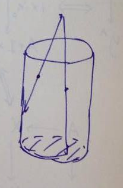
\includegraphics[scale=0.75]{retract-cofibration}
	\caption{Drawing by John Ni.}
    \end{figure}
\end{example}
In particular, $\{0,1\}\hookrightarrow I$ is a cofibration.
\chapter{Homotopy fibers, the Barratt-Puppe sequence}
Yesterday, I showed this:
\begin{prop}
    If $A\to X$ is a cofibration, then for any $Y$, the map $Y^X\to Y^A$ is a fibration.
\end{prop}
We did this by reverse-engineering.
\begin{example}
    $S^{n-1}\hookrightarrow D^n$ is a cofibration.
\end{example}
Let me point out properties of cofibrations.
\begin{itemize}
    \item It's closed under cobase change. What this means is if I have a cofibration $A\to X$ and any $A\to B$, then $B\to X\cup_A B$ is a cofibration.
    \item It's closed under finite products. This is surprising.
    \item It's closed under composition.
    \item Any cofibration is a closed inclusion. This is not so obvious, so check out May's book.
\end{itemize}
By the way, the dual statement would be something like: $p:E\to B$ a quotient map? No! Fibrations don't have to be surjective at all. It is surjective on path components though, because of the path-lifting stuff. But, for example, $\emptyset\to B$ is a fibration.

Another fact on fibrations is that $X\to \ast$ is a fibration, because the dotted map can be taken to the map $(t,w)\mapsto f(w)$:
\begin{equation*}
    \xymatrix{
    W\ar[d]\ar[r]^f & X\ar[d]\\
    I\times W\ar@{-->}[ur]\ar[r] & \ast
}
\end{equation*}
Model category folks get excited about this, because this says that all objects in the model structure on topological spaces is fibrant. 
\begin{definition}
Now, the inclusion $\ast\hookrightarrow X$ is not always a cofibration (see your pset!), but if it is, say that $\ast$ is a nondegenerate basepoint in $X$.
\end{definition}
Eg if $\ast$ has a neighborhood that contracts to $\ast$ then $\ast\hookrightarrow X$ is a cofibration. If $\ast$ is a nondegenerate basepoint, then $X^A\xrightarrow{ev} X$ is a fibration where $A$ is pointed. The fiber is the space of pointed maps $A\to X$.

Because $S^{n-1}\hookrightarrow D^n$ is a cofibration, we find that $\{0,1\}\hookrightarrow I$ is a cofibration. This means that the map $Y^I\to Y\times Y$ given by $\omega\mapsto (\omega(0),\omega(1))$ is a fibration. This gets into the story of path spaces.
\section{''Fibrant replacements''}
Don't worry about the title of this section. If you've seen model categories, this'll make sense.
\begin{theorem}
    Any map is $\simeq$ to a fibration. What does this mean? This means that for any map $f:X\to Y$ we can find a space $T(f)$ such that:
    \begin{equation*}
	\xymatrix{
	    X\ar[dr]^{\simeq}\ar[d]_f & T(f)\ar[d]^p\\
	    & Y
	    }
    \end{equation*}
    where $p$ is a fibration and $X\xrightarrow{\simeq} T(f)$ is a homotopy equivalence.
\end{theorem}
\begin{proof}
    Consider the map $Y^I\xrightarrow{\begin{pmatrix} ev_0 \\ ev_1\end{pmatrix}}Y\times Y$. Define $T(f)$ as the pullback:
	\begin{equation*}
	    \xymatrix{
		T(f)\ar[r]\ar[d] & Y^I\ar[d]^{\begin{pmatrix}ev_0 \\ ev_1\end{pmatrix}}\\
		    X\times Y\ar[r]_{f\times 1} & Y\times Y
		}
	\end{equation*}
	In other words, $T(f)=\{(x,\omega)\in X\times Y^I|f(x) = \omega(0)\}$. Let's start checking the conditions. First of all, the map $Y^I\to Y\times Y$ is a fibration. So $T(f)\to X\times Y$ is a fibration. Since $X\times Y\to Y$ is a fibration, we can consider the composite $T(f)\to X\times Y\to Y$, which is now a fibration. On elements, $T(f)\to Y$ sends $(x,\omega)\to \omega(1)$.

	To get a map $X\to T(f)$, I need to give maps $X\to X\times Y$ and $X\to Y^I$ that have compatible images in $Y\times Y$. Define $X\to X\times Y$ as $X\xrightarrow{\begin{pmatrix} 1 \\ f\end{pmatrix}}X\times Y$, and define $X\to Y^I$ as the map sending $x$ to the constant loop at $f(x)$. Clearly both composite $X\to X\times Y\\to Y\times Y$ and $X\to Y^I\to Y\times Y$ are the same, so we have a map $X\to T(f)$.

	    Is it true that the composite $X\to T(f)\xrightarrow{p} Y$ is our original map? Yes! So we only have to check that $X\to T(f)$ is a homotopy equivalence. Let me begin by constructing a homotopy inverse. I.e., a map $T(f)\to X$. We can define a map $T(f)\to X$ via $T(f)\to X\times Y\xrightarrow{pr_1} X$. Clearly the composite $X\to T(f)\to X\times Y\to X$ is the identity. This means we need to study $T(f)\to X\to T(f)$. This composite sends $(x,\omega)\mapsto x\mapsto (x,c_{f(x)})$ where $c_{f(x)}$ is the constant path at $x$. I need a homotopy between this map and the identity on $T(f)$.

	    This is what I call the spaghetti move. We know that there's no constraint on $\omega(1)$, so I can just suck it back in to get the constant loop. I guess I can define $\omega_s(t) = \omega(st)$. At $s=1$ I have $\omega$ and when $s=0$ I have $c_{f(x)} = c_{\omega(0)}$. Thus, define $I\times T(f)\to T(f)$ via $(s,(x,\omega))\mapsto (x,\omega_s)$.

	    If you want to work through the diagram, this is how it looks.
	    \begin{equation*}
		\xymatrix{
		    X\ar@{-->}[dr]\ar[drr]^{x\mapsto c_{f(x)}}\ar[ddr]_{\begin{pmatrix}1 \\ f\end{pmatrix}} & & \\
			& T(f)\ar[d]\ar[r]\ar[dr] & Y^I\ar[d]^{\begin{pmatrix}ev_0 \\ ev_1\end{pmatrix}}\\
			    X & X\times Y\ar[l]^{pr_1}\ar[d]^{pr_2}\ar[r] & Y\times Y\\
		    & Y
		    }
	    \end{equation*}
\end{proof}
Here's a really stupid example. 
\begin{example}[Path-loop fibration]
Suppose $X=\ast$. What is $T(f)$? Well it's just paths $\omega(0)$ in $Y$ such that $\omega(0)=\ast$. I.e., $T(f) = Y^I_\ast$. This is also called the path space of $Y$, denoted $P(Y,\ast)$. It's contractible by the spaghetti move. What it's fiber? The map $PY\to Y$ sends $\omega\mapsto \omega(1)$. So the fiber is the points that begin at $\ast$ and end at $\ast$. The fiber of $PY\to Y$ is denoted $\Omega Y$, which is the space of loops at $\ast$. This is called the path loop fibration. 
\end{example}
\section{Homotopy fibers over $\ast$}
The ordinary fiber is the pullback
\begin{equation*}
    \xymatrix{
	f^{-1}(\ast)\ar[r]\ar[d] & X\ar[d]^f\\
	\ast\ar[r] & Y
    }
\end{equation*}
\begin{definition}[Homotopy fiber]
    The homotopy fiber is the pullback:
    \begin{equation*}
	\xymatrix{
	    F(f,\ast)\ar[r]\ar[d] & T(f)\ar[r]\ar[d]^p & X\ar[dl]^f\\
	    \ast \ar[r] & Y &
	    }
    \end{equation*}
\end{definition}
As a set it's $F(f,\ast) = \{(x,\omega)\in X\times Y^I| f(x) = \omega(0), \omega(1) = \ast\}$. The ordinary fiber and the homotopy fiber are definitely not generally the same. If $W\to X\to Y$ is nullhomotopic, then it factors through $F(f,\ast)$, i.e., the composite factors as $W\to F(f,\ast)\to X\to Y$.
\begin{prop}
    Suppose $p:X\to Y$ is a fibration. Let $\ast\in Y$. Then $p^{-1}(\ast)\to F(p,\ast)$ is a homotopy equivalence.
\end{prop}
I'm not going to prove that, but you will for homework.

A different way to construct the homotopy fiber is to replace $f:X\to Y$ by a fibration. But what if I replace $\ast\to Y$ by a fibration? Namely, we now have:
\begin{equation*}
    \xymatrix{
	??\ar[r]\ar[d] & P(Y,\ast)\ar[r]^{\simeq} & \ast\ar[dl]\\
	X\ar[r] & Y & 
    }
\end{equation*}
This space $??$ consists of $(x,\omega)\in X\times Y^I$ such that $\omega(0) = \ast$ and $\omega(1) = f(x)$. Now, $F(f,\ast) = \{(x,\omega):\omega(0) = f(x), \omega(1) = \ast\}$. So $??$ is homeomorphic to $F(f,\ast)$ by reversing directions of paths. There's two ways you can produce a homotopy fiber, and all of these are homeomorphic. You could also replace both of these maps $f$ and $\ast\to Y$ by a fibration, and you'll get something that's also homeomorphic. Note that when I say $F(f,\ast)$, I'll mean $??$.

Here's what you'll prove for homework.
\begin{theorem}
    Suppose you have two fibrations $p$ and $p^\prime$ such that the following diagram commutes, where $f$ is a homotopy equivalence.
    \begin{equation*}
	\xymatrix{
	    E\ar[r]^p\ar[dr]^p & E^\prime\ar[d]^{p^\prime}\\
	    & B
	    }
    \end{equation*}
    Then $f$ is a fiber homotopy equivalence. That means that it's a homotopy equivalence in $\Top_{/B}$. What this means is that there is a map $g:E^\prime\to E$ over $B$ compatible with the fibrations and homotopies $I\times E\to E$ over $B$ and $I\times E^\prime\to E^\prime$ over $B$. I.e., the following three diagrams commute:
    \begin{equation*}
	\xymatrix{
	    E^\prime\ar[r]^g\ar[dr]^{p^\prime} & E\ar[d]^p\\
	    & B
	    }
    \end{equation*}
    and 
    \begin{equation*}
	\xymatrix{
	    I\times E\ar[r]^{1\sim gf}\ar[dr] & E\ar[d]^p\\
	    & B
	    }
    \end{equation*}
    and
    \begin{equation*}
	\xymatrix{
	    I\times E^\prime\ar[r]^{1\sim fg}\ar[dr] & E^\prime\ar[d]^{p^\prime}\\
	    & B
	    }
    \end{equation*}
\end{theorem}
So we find that for all $b$, $p^{-1}(b)\xrightarrow{\simeq} (p^\prime)^{-1}(b)$. So in particular, the fiber $F(f,\ast)$, i.e., the homotopy fiber, of $T(f)\to B$ and the fiber $f^{-1}(\ast)$ of $f:E\to B$ are homotopy equivalent if $f$ is a fibration.
\chapter{Barratt-Puppe sequence, $\pi_\ast$}
Hood's office hours are from 12 to 1:30 on Mondays in 2-390. Mine are from 4-5 on Tuesday in 2-478. Hood's graded the homework already.
\section{Fiber sequences}
Recall we have a pullback diagram:
\begin{equation*}
    \xymatrix{
	& F(f,\ast)\ar[r]\ar[d]^p & PY\ar[d]^p\ar[dr]^{\simeq} & \\
	f^{-1}(\ast)\ar[ur]\ar[r] & X\ar[r]_f & Y & \ast\ar[l]
    }
\end{equation*}
The homotopy fiber $F(f,\ast)$ thus has elements $\{(x,\sigma)\in X\times PY| f(x) = \sigma(1)\}$. We also have the ordinary fiber $f^{-1}(\ast)$. If $f$ is a fibration, the canonical map $f^{-1}(\ast)\to F(f,\ast)$ sending $x\mapsto(x,c_{f(x)})$ is a homotopy equivalence.
\begin{remark}
Consider a pointed map\footnote{Some people say ``based maps'', but it sounds like chemistry ... or evil, so I can't bring myself to say it} $f:X\to Y$, i.e., $f(\ast) = \ast$. Then I'll write $Ff$ for $F(f,\ast)$.
\end{remark}
Ok, what's the fiber of $p:Ff\to X$? The fiber over the basepoint in $X$ is precisely the space of loops in $Y$! I.e., $p^{-1}(\ast_X) = \Omega Y$, which is the space of loops in $Y$ based at $\ast_Y$. Note that this is also the homotopy fiber because $p$ is a fibration (fibrations are closed under pullbacks). So the diagram we now have is:
\begin{equation*}
\xymatrix{\\
    & \Omega Y=p^{-1}(\ast)\ar[d] & & &\\
    & F(f,\ast)\ar[r]\ar[d]^p & PY\ar[d]^p\ar[dr]^{\simeq} & \\
    f^{-1}(\ast)\ar[ur]\ar[r] & X\ar[r]_f & Y & \ast\ar[l]
}
\end{equation*}
The composite $Ff\to X\to Y$ sends $(x,\omega)\mapsto f(x)$. This is a pointed map, but not equal to the constant map. What does this even mean? Like, what is the basepoint we're choosing for $Ff$? Well, choose the basepoint to be the image of the basepoint in $f^{-1}(\ast)$ under $f^{-1}(\ast)\hookrightarrow Ff$.

We also have a (pointed!) homotopy between $Ff\to X\to Y$ and the constant map, eg via $h:Ff\times I\to Y$ defined by $h(t,(x,\omega)) = \omega(t)$. We say that the composite is \emph{nullhomotopic}. In fact, suppose $W\to X\to Y$ is nullhomotopic, with a chosen nullhomotopy -- this is the same as a map $W\to Ff$. This is a question on your homework.

Let's write $[W,X]_\ast = \pi_0(X^W_\ast)$, i.e., the pointed homotopy classes of maps $W\to X$. This is a pointed set, whose basepoint is the constant map. Ok, I can consider $[W,Ff]_\ast\to [W,X]_\ast\to [W,Y]_\ast$. This composite is nullhomotopic. But I want to say that this sequence is exact. What that means is here (because we just have pointed sets). So the preimage of the basepoint in $[W,Y]_\ast$ equals the image of $[W,Ff]_\ast\to [W,X]_\ast$. This is exactly what I said before, about nullhomotopies $W\to X\to Y$ as maps $W\to Ff$. We say that $Ff\to X\xrightarrow{f}Y$ is a \emph{fiber sequence}.

\section{Iterating fiber sequences}
I have $Ff\xrightarrow{p} X\xrightarrow{f} Y$. The strict fiber is $\Omega Y$, but the homotopy fiber is $Fp$. These are homotopy equivalent because $p$ is a fibration. Denote the map $i:\Omega Y\to Ff$. This sits inside:
\begin{equation*}
    \xymatrix{
	\cdots\ar[r] & Fp_3 \ar[r] & Fp_2\ar[r] & Fp_1\ar[r]^{p_2} & Ff\ar[r]^{p_1} & X\ar[r]^{f} & Y\\
	& \Omega Fp_0\ar[u]_{\simeq}\ar[ur]|{i(p_2)}\ar@{-->}[r] & \Omega X\ar@{-->}[r]\ar[u]_{\simeq}\ar[ur]|{i(p_1)} & \Omega Y\ar[u]_\simeq \ar[ur]|{i(p_0)} & &
    }
\end{equation*}
All the $p_i$s are fibrations (think about why). The dotted maps seem to be missing; I can fill them in up to homotopy, and there's one map I can think of putting there: $\Omega X\xrightarrow{\Omega f}\Omega Y$. But \emph{that's the wrong map}! The right map is $\Omega X\xrightarrow{\overline{\Omega f}}\Omega Y$ (see below for explanation). Here's a lemma.
\begin{lemma}
    The following diagram commutes to homotopy:
    \begin{equation*}
	\xymatrix{
	    & Fp\\
	    \Omega X\ar[r]_{\overline{\Omega f}}\ar[ur]^{i(p)} & \Omega Y\ar[u]
	    }
    \end{equation*}
    where $\overline{\Omega f}$ is the diagonal in:
    \begin{equation*}
	\xymatrix{
	    \Omega X\ar[r]^{-}\ar[dr]|{\Omega f} \ar[d]_{\Omega f} & \Omega X\ar[d]^{\Omega f}\\
	    \Omega Y\ar[r]_{-} & \Omega Y
	    }
    \end{equation*}
    where $-:\Omega X\to \Omega X$ sends $\omega\mapsto\overline{\omega}$.
\end{lemma}
\begin{proof}
    There is a beautiful proof of this. But it's in pictures, and I can't type it. The main point is that the proof wouldn't work unless you moved backwards. See this image:
\begin{figure}[H]
\centering
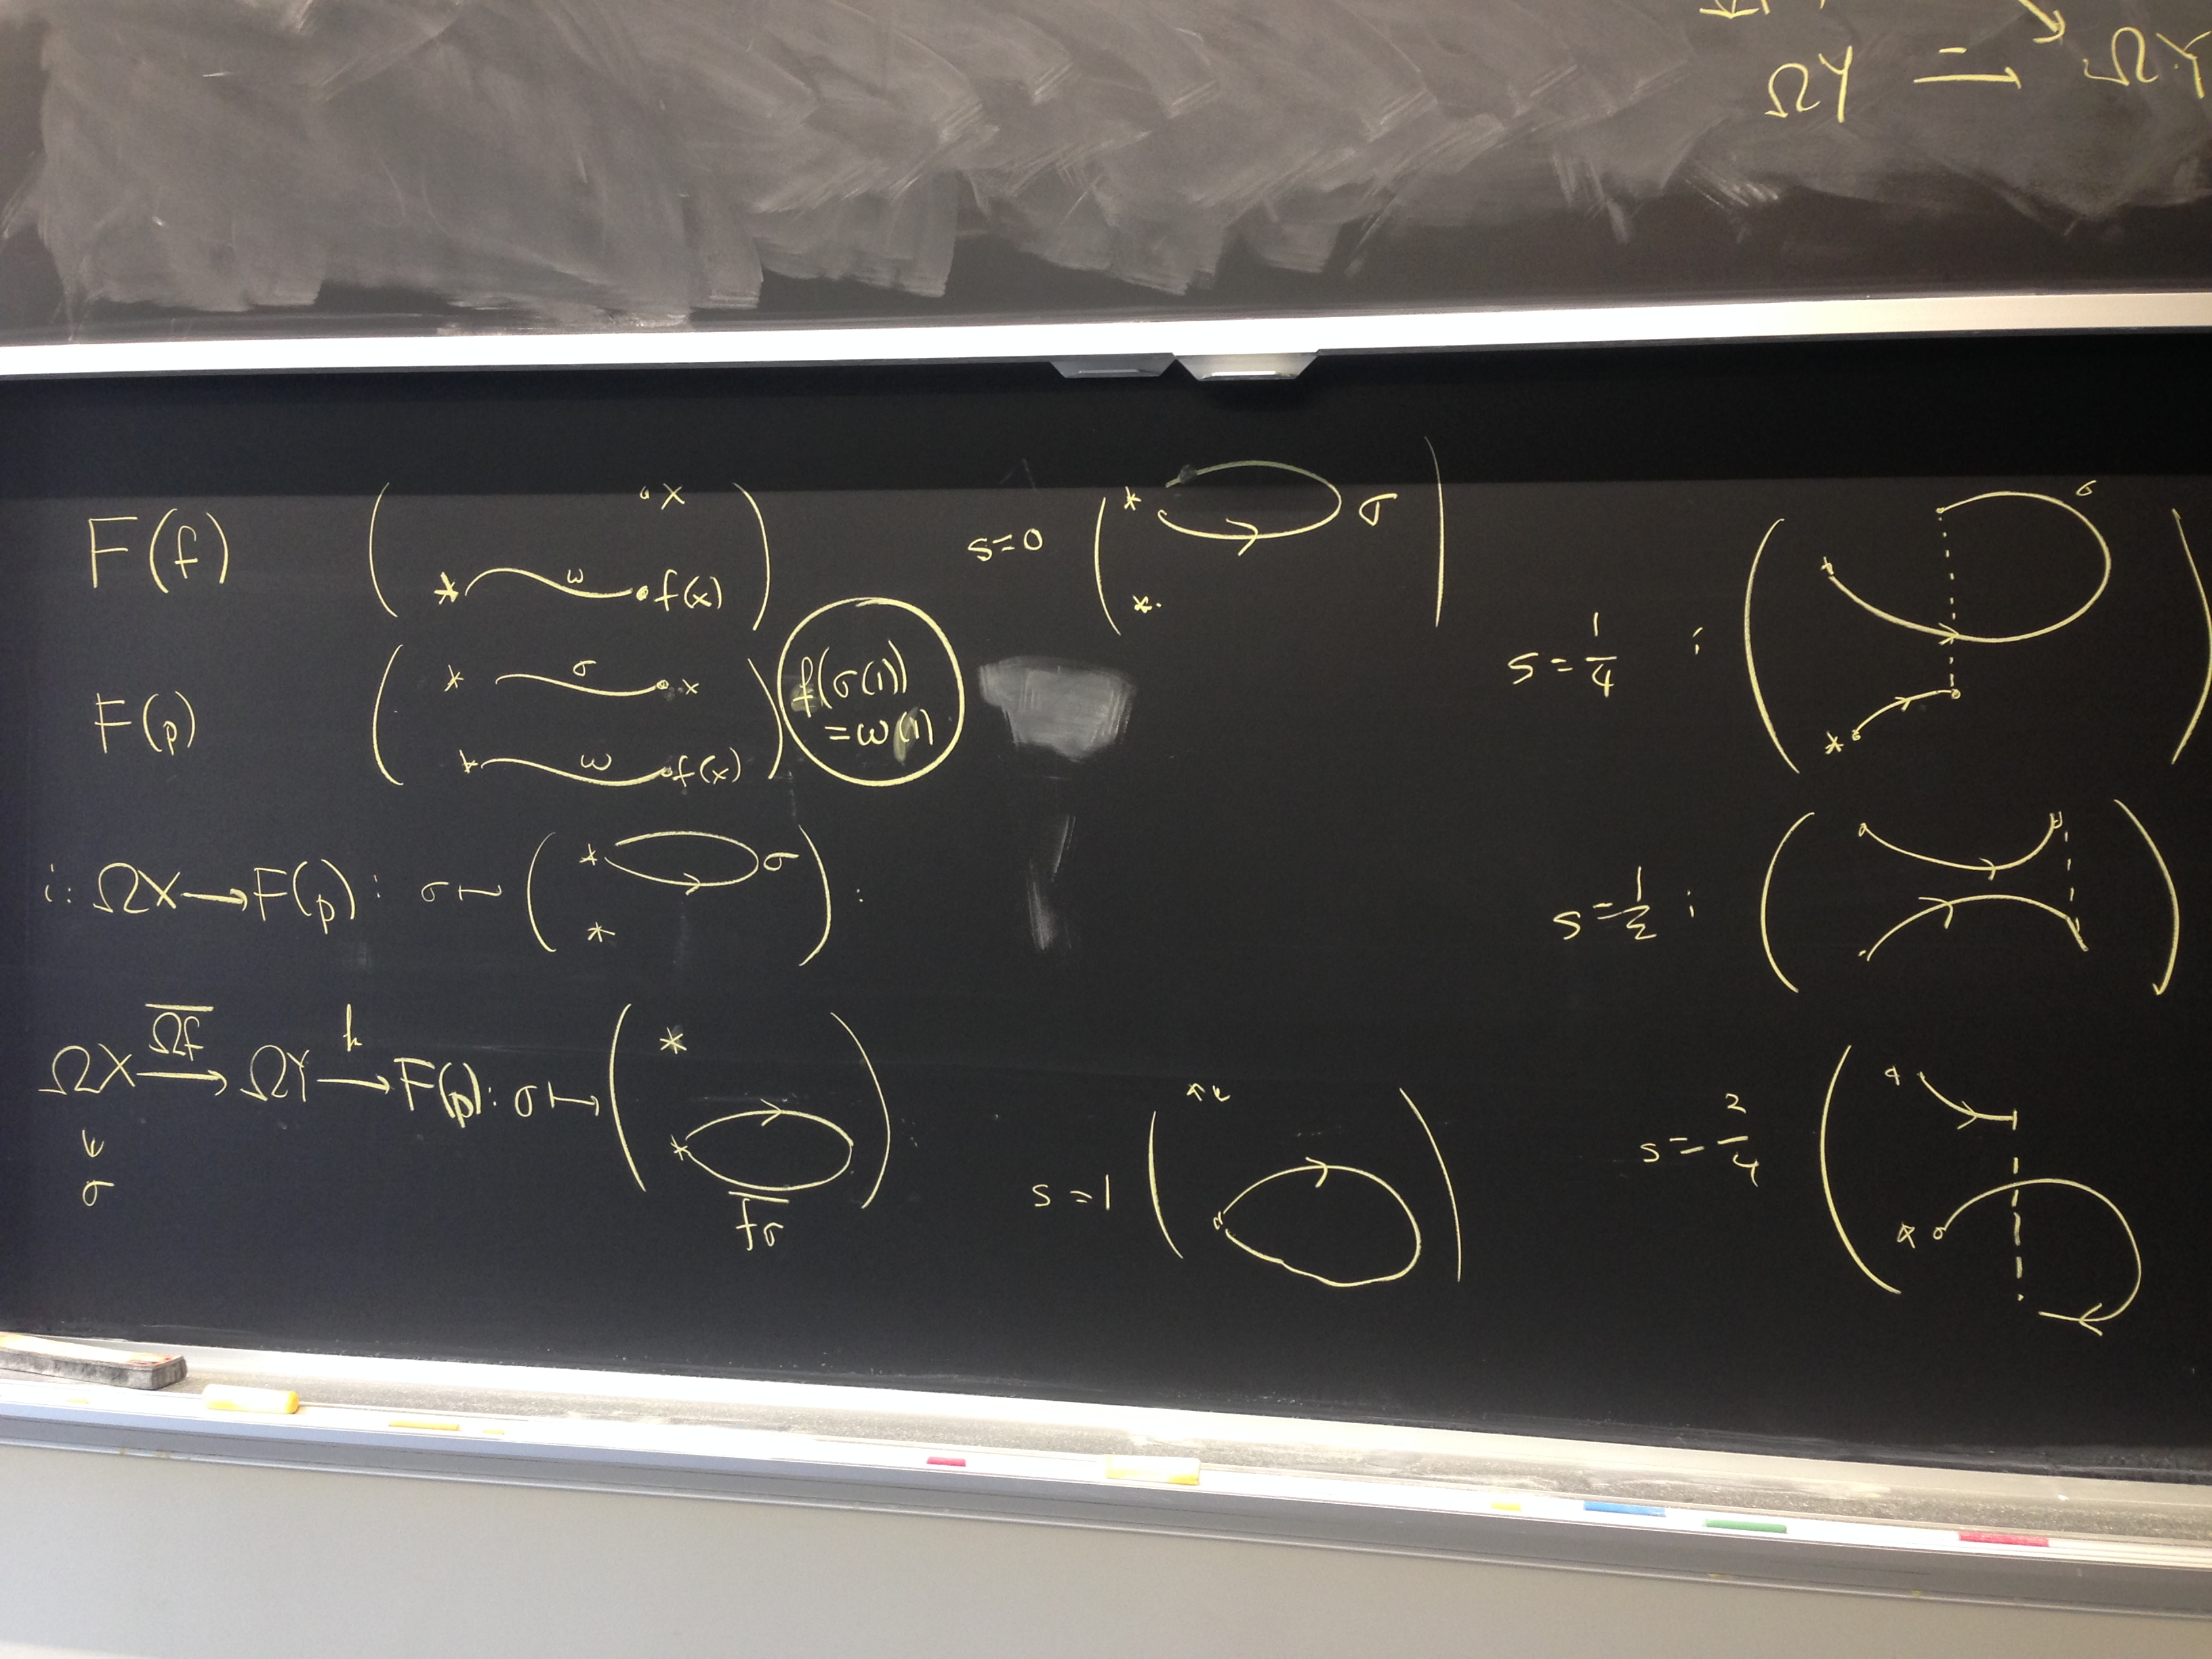
\includegraphics[width=\textwidth]{barratt-puppe}
\caption{A proof of this lemma.}
\end{figure}
\end{proof}
\begin{lemma}
    The following diagram commutes:
    \begin{equation*}
	\xymatrix{
	    & F(\overline{\Omega p_0})\ar@{=}[dd]\ar[dr] & \\
	    \Omega^2 Y\ar[ur]^{i(\Omega p_0)}\ar[dr]_{\overline{\Omega i(p_0)}} & & \Omega X\\
	    & \Omega Fp_0\ar[ur]_{\overline{\Omega p_1}} & 
	    }
    \end{equation*}
\end{lemma}
What is the map $F\overline{\Omega p_0}\to \Omega X$?? We spent some time figuring this out. But you can now apply $[W,-]_\ast$ to the following diagram to get a long exact sequence:
\begin{equation*}
    \xymatrix{
	\cdots\ar[r] & Fp_4\ar[r] & Fp_3 \ar[r] & Fp_2\ar[r] & Fp_1\ar[r]^{p_2} & Ff\ar[r]^{p_1} & X\ar[r]^{f} & Y\\
    \cdots\ar[r] & \Omega Fp_1\ar[r]|{\overline{\Omega p_2}}\ar[u]_{\simeq} & \Omega Fp_0\ar[u]_{\simeq}\ar[ur]|{i(p_2)}\ar[r]|{\overline{\Omega p}} & \Omega X\ar[r]|{\overline{\Omega f}}\ar[u]_{\simeq}\ar[ur]|{i(p_1)} & \Omega Y\ar[u]_\simeq \ar[ur]|{i(p_0)} & &\\
	\Omega^2 X\ar[u]_{\simeq}\ar[r]_{\Omega f} & \Omega Y\ar[u]_{\simeq}\ar[ur]_{\overline{\Omega i(p_0)}} & & &
    }
\end{equation*}

For example, $S^0=\{\pm 1\}$. We get terms like $\pi_0(\Omega^n X)$, because $[S^0,X] = \pi_0 X$. What is $\pi_0(\Omega^n X)$? This is $[S^0,\Omega^n X]_\ast$. Is it clear to you that this is $[S^n,X]_\ast$?

Ok, well, $\Omega^2 X = (\Omega X)^{S^1}$. Because $(S^1)^{\wedge n} = S^n$. So we find that $(\Omega X)^{S^1} = (X^{S^1}_\ast)^{S^1}_\ast = X_\ast^{S^1\wedge S^1} = X_\ast^{S^2}$.

Well, $\Omega X$ is a homotopy group by concatenation. It's a group, but where the axioms hold up to homotopy. It's a group in the homotopy category. Therefore, $\pi_0 \Omega X$ is a group! It's exactly $\pi_1 X$, which you know to be a group. And then, there's this other thing that happens.

You can think of $\pi_n(X) = [S^n,X]_\ast$ as $[(D^n,S^{n-1}),(X,\ast)] = [(I^n,\partial I^n),(X,\ast)]$. If I take $n=2$, for example, how do I take the product of $\alpha,\beta\in \pi_2(X)$? You just literally put them together (when you think of $\pi_2(X) = [(I^2,\partial I^2),(X,\ast)]$. You can play this game; up to homotopy, you can shrink $\alpha$ and $\beta$ to make them as small I want, and then reverse their position and expand them again\footnote{This probably makes no sense without a picture}\todo{Add a picture}. Thus $\pi_2(X)$ is an abelian group.

Thus, when you apply $\pi_0$ to our sequence $\cdots\to\Omega^2 X\to\Omega^2 Y\to \Omega Fp_0\to \Omega X\to \Omega Y\to Fp_0\to \Omega X\to \Omega Y$, you get an exact sequence (of groups when the homotopy groups are $>0$, and of pointed sets when you have $\pi_0$):
$$\cdots\to \pi_2 X\to \pi_2 Y\to \pi_1 Ff\to \pi_1 X\to\pi_1 Y\to\pi_0 Ff\to\pi_0 X\to \pi_0 X$$
\chapter{Relative homotopy, $\pi_1$ action}
Pset 2 has question 8; there's still one more to go. Hood has office hours today 12 -- 1 in 2-390, and I have office hours today tomorrow 4-5 in 2-478.
\section{Spheres and homotopy groups}
Let's talk about spheres, first of all. The $n$-sphere is $S^n=I^n/\partial I^n$. Agreed? It's a standard choice. By the way, $S^1 = I/0\sim 1$. What about $S^0$? This is $\ast/\emptyset = \ast_+$. This is the usual way to think of the zero sphere. The point that you just added is the basepoint.

We have this looping thing going on; we know that $\Omega X$ (I'm always working in $\Top_\ast$ these days) is $X^{S^1}_\ast$. Thus the adjunction says that $\Top_\ast(W,\Omega X) = \Top_\ast(S^1\wedge W,X)$.
\begin{definition}
    The \emph{reduced suspension} $\Sigma W$ is $S^1\wedge W$.
\end{definition}
If I have $A\subseteq X$, then $X/A\wedge Y/B = (X\times Y)/((A\times Y)\cup_{A\times B}(X\times B))$. Thus $\Sigma X = S^1\wedge X$ is $I\times X/(\partial I \times X\cup I\times \ast)$. I collapse the top and bottom of a cylinder to a point, and also the line along a basepoint gets collapsed.

Similarly, $\Sigma^n X$ is the left adjoint of the $n$-fold loop space. Hence $\Sigma^n X = (S^1)^{\wedge n}\wedge X$. What is $S^1\wedge S^n$? This is $I/\partial I\wedge I^n\wedge \partial I^n = (I\times I^n)/(\partial I\times I^n\cup I\times \partial I^n)$. This denominator is exactly $\partial I^{n+1}$; hence $S^1\wedge S^n\simeq S^{1+n}$. In fact, $S^k\wedge S^n\simeq S^{k+n}$.
\begin{definition}
    The $n$th homotopy group of $X$ is $\pi_n X = \pi_0(\Omega^n X)$.
\end{definition}
This is $[S^0,\Omega^n X]_\ast = [S^n, X]_\ast = [(I^n,\partial I^n),(X,\ast)]$.
\section{The homotopy category}
We have the \emph{homotopy category of spaces} $\Ho(\Top)$ whose objects are spaces and whose mapping spaces are $\pi_0$ of mapping spaces. I have to check that if $f_0,f_1:X\to Y$ and $g:Y\to Z$, then $gf_0\simeq gf_1$. Of course, it is, just by composing with $g$. Similarly $f_0h\simeq f_1h$. This guarantees that you can define composition of maps in $\Ho(\Top)$. I can also think about $\Ho(\Top_\ast)$, with pointed homotopies. A lot of what we've been doing has been taking place in $\Ho(\Top_\ast)$.

Fix $W$. We need to check that $X\mapsto X^W_\ast$ is a homotopy functor. It defines a functor $\Top_\ast\to\Top_\ast$. Namely, I want to complete:
\begin{equation*}
    \xymatrix{
	\Top_\ast\ar[d]\ar[r]^{X\mapsto X^W_\ast} & \Top_\ast\ar[d]\\
	\Ho(\Top_\ast)\ar@{-->}[r] & \Ho(\Top_\ast)
    }
\end{equation*}
So I'd better check that if I have a homotopy $f_0\sim f_1:X\to Y$. Is that a map $I\wedge X\to Y$? This really tells you that there's a nullhomotopy if the basepoint of $I$ is one of the endpoints. I really want to consider $I\times X/I\times\ast$. Aha, but this is just $I_+\wedge X$. So a homotopy $f_0\sim f_1:X\to Y$ is a map $I_+\wedge X\to Y$.

Suppose I have a homotopy like this; then I get $(I_+\wedge X)^W\to Y^W_\ast$. I wanted $I_+\wedge X^W_\ast\to Y^W_\ast$, so that's not quite what I wanted. I can get this if I can construct a map $I_+\wedge X^W_\ast\to (I_+\wedge X)^W_\ast$. In fact, I want to construct $A\wedge X^W_\ast\to (A\wedge X)^W_\ast$. One thing I can do is $A\wedge X^W_\ast\to A^W_\ast\wedge X^W_\ast$ by sending $a\mapsto c_a$, and then the exponential law gives a homotop $A^W_\ast\wedge X^W_\ast\to (A\wedge X)^W_\ast$. This gives me a map $I_+\wedge X^W_\ast\to (I_+\wedge X)^W_\ast\to Y^W_\ast$ making $X\mapsto X^W_\ast$ a homotopy functor. In particular, $\Omega^n$ is a homotopy functor.

Let's continue with this homotopical localization of things.
\begin{definition}
    A fiber sequence in $\Ho(\Top_\ast)$ is a composite $X\to Y\to Z$ that is isomorphic in $\Ho(\Top_\ast)$ to some $Ff\xrightarrow{p} E\xrightarrow{f}B$. Namely we want some (possibly zig-zag of) maps that are homotopy equivalences:
    \begin{equation*}
	\xymatrix{
	    X\ar[r]\ar[d] & Y\ar[r]\ar[d] & Z\ar[d]\\
	    Ff\ar[r]_p & E\ar[r]_f & B
	    }
    \end{equation*}
\end{definition}
We've seen examples in our elaborate story. Recall our diagram:
\begin{equation*}
    \xymatrix{
	\cdots\ar[r] & Fp_4\ar[r] & Fp_3 \ar[r] & Fp_2\ar[r] & Fp_1\ar[r]^{p_2} & Ff\ar[r]^{p_1} & X\ar[r]^{f} & Y\\
    \cdots\ar[r] & \Omega Fp_1\ar[r]|{\overline{\Omega p_2}}\ar[u]_{\simeq} & \Omega Fp_0\ar[u]_{\simeq}\ar[ur]|{i(p_2)}\ar[r]|{\overline{\Omega p}} & \Omega X\ar[r]|{\overline{\Omega f}}\ar[u]_{\simeq}\ar[ur]|{i(p_1)} & \Omega Y\ar[u]_\simeq \ar[ur]|{i(p_0)} & &\\
	\Omega^2 X\ar[u]_{\simeq}\ar[r]_{\Omega f} & \Omega Y\ar[u]_{\simeq}\ar[ur]_{\overline{\Omega i(p_0)}} & & &
    }
\end{equation*}
So look, $Ff\to X\to Y$ is a fiber sequence. And $\Omega Y\to F\xrightarrow{p}X$ is another fiber sequence because it's isomorphic to $Fp\to F\to X$ in $\Ho(\Top_\ast)$. I also have $\Omega X\xrightarrow{\overline{\Omega f}}\Omega Y\to F$ is another fiber sequence. This means that $\Omega X\xrightarrow{\Omega f}\Omega Y\to F$ is another fiber sequence because these two fiber sequences differ by an automorphism of $\Omega X$ because in general, if $A^\prime\xrightarrow{\sim} A$ and $A\to B\to C$ is a fiber sequence, so is $A^\prime\xrightarrow{\sim} A\to B\to C$.

I can apply $\Omega$ again, so I get $\Omega F\xrightarrow{\Omega p} \Omega X\xrightarrow{\Omega f} \Omega Y$. I claim this is a fiber sequence, because this is a loop of a fiber sequence, and taking loops takes fiber sequences to fiber sequences. This is called the \emph{Barratt-Puppe sequence}. I carefully explained that this makes some sense, because it firstly makes sense to ask that $\Omega$ is a homotopy functor. I haven't said this yet. So in particular:
\begin{enumerate}
    \item $\Omega$ takes fiber sequences to fiber sequences.
    \item $\Omega Ff\simeq F\Omega f$. Check this!
\end{enumerate}
You can now \emph{loop back} to get $\Omega^2 Y\xrightarrow{\Omega i} \Omega F\xrightarrow{\Omega p}\Omega X$. This is an unstable version of a triangulated category. It wants to be a triangulated category, but it isn't.
\begin{remark}
    If $f:X\to Y$, I can form $Ff$. I might have a homotopy commuting diagram like:
    \begin{equation*}
	\xymatrix{
	    \Omega Y\ar[d]_{\Omega g}\ar[r] & Ff\ar@{-->}[d]\ar[r] & X\ar[d]_{h}\ar[r]^f & Y\ar[d]^g\\
	    \Omega Y^\prime\ar[r] & Ff^\prime\ar[r] & X^\prime\ar[r]_{f^\prime} & Y
	    }
    \end{equation*}
    The dotted map exists, but \emph{this map depends on the homotopy} $f^\prime h\simeq gf$. That's an important subtlety.
\end{remark}
\section{lexseq of a fiber sequence}
Applying $\pi_0 = [S^0,-]_\ast$ to the Barratt-Puppe sequence gives a lexseq:
\begin{equation*}
    \xymatrix{
	& \cdots\ar[r] & \pi_2 Y\ar[dll]\\
	\pi_1 F\ar[r] & \pi_1 X\ar[r] & \pi_1 Y\ar[dll]\\
	\pi_0 F\ar[r] & \pi_0 X\ar[r] & \pi_1 X
    }
\end{equation*}
of pointed sets. But this is even better, ,because $\Omega X$ is a group object in $\Ho(\Top_\ast)$.
\begin{remark}
    $\Ho(\Top)$ and $\Ho(\Top_\ast)$ has products and coproducts, but very few other limits or colimits. So as a category, it is \emph{horrible}.
\end{remark}
I showed you an argument that $\Omega^2 X$ is an \emph{abelian} group object, i.e., multiplication is commutative up to homotopy. Thus $\pi_1$ is a group and $\pi_k$ is an abelian group for $k\geq 2$; hence in our diagram above, all maps (except on $\pi_0$) are group homomorphisms!

What if $X\to Y$ is the inclusion $i:A\hookrightarrow X$ of a subspace? Then $Fi=\{(a,\omega)\in A\times X^I_\ast|\omega(1) = a\}$. This is just the collection of all paths that begin at $\ast\in A$ and ends in $A$.
\begin{definition}
    $\pi_n(X,A,\ast) = \pi_n(X,A)$ is $\pi_{n-1}Fi = [(I^n,\partial I^n,(\partial I^n\times I)\cup (I^{n-1}\times 0)),(X,A,\ast)]$.
\end{definition}
Inside $I^n$ is $\partial I^n$, and also including in it is $\partial I^n\times I\cup I^{n-1}\times 0$. Then you can check that $\pi_{n-1}Fi = [(I^n,\partial I^n,(\partial I^n\times I)\cup (I^{n-1}\times 0)),(X,A,\ast)]$. In this case, you have a lexseq: 
\begin{equation*}
    \xymatrix{
	& \cdots\ar[r] & \pi_2 (X,a)\ar[dll]\\
	\pi_1 A\ar[r] & \pi_1 X\ar[r] & \pi_1 (X,A)\ar[dll]\\
	\pi_0 A\ar[r] & \pi_0 X\ar[r] & 
    }
\end{equation*}
